\section{Cryptanalysis}

\begin{frame}{Differential Attack}
\begin{block}{}
    \begin{itemize}
        \item Differential Cryptanalysis is one of the strongest techniques for the cryptanalysis of block ciphers.
        \item Using the algorithm based on the branch and bound method, the best differential trails from round-1 to round-15 were found.
        \begin{block}{}
            \tiny
            \centering
            \begin{array}{||c|c||c|c||c|c||}
                \hline \sharp R & \text { Prob. } & \sharp \mathrm{R} & \text { Prob. } & \sharp \mathrm{R} & \text { Prob. } \\
                \hline 1 & 2^{-2} & 6 & 2^{-18} & 11 & 2^{-46} \\
                \hline 2 & 2^{-4} & 7 & 2^{-25} & 12 & 2^{-51} \\
                \hline 3 & 2^{-7} & 8 & 2^{-31} & 13 & 2^{-56} \\
                \hline 4 & 2^{-10} & 9 & 2^{-36} & 14 & 2^{-61} \\
                \hline 5 & 2^{-14} & 10 & 2^{-41} & 15 & 2^{-66} \\
                \hline
            \end{array}
        \end{block}
        \item Using the 14-round differential propagation, we can mount an attack on the 18-round Rectangle cipher.
        \item A 25-round Rectangle cipher is sufficient to withstand this differential cryptanalysis attack.
    \end{itemize}
        
\end{block}
\end{frame}

\begin{frame}{Integral Attack}
\begin{block}{}
    \begin{itemize}
        \item Implemented Square Attack, which uses a 4-round integral distinguisher.
        \item After 4 rounds, the XOR sum in any 4-bit positions equals 0, i.e., the balanced property:
        \[
        \oplus S_{(0,0)} = \oplus S_{(1,1)} = \oplus S_{(2,13)} = \oplus S_{(3,13)} = 0
        \]
        \item Visual Representation:
        \begin{figure}[h!]
            \centering
            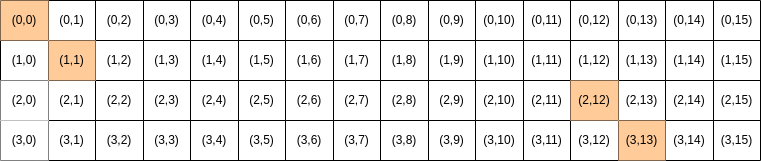
\includegraphics[width=0.6\textwidth]{diff1.drawio.png} % Replace with your image filename
            \label{fig:integral_attack}
        \end{figure}
        \item Decryption: We choose 248 plaintexts such that:
        \begin{itemize}
            \item Columns 0, 13, 14, 15 maintain the CONSTANT property.
            \item Other 12 columns maintain the **ALL** property.
        \end{itemize}
        \item $2^{48}$ Intermediate values $\implies 2^{47}$ subsets $\implies 2$ values.
    \end{itemize}
        
\end{block}
\end{frame}

